\documentclass[oneside,final,12pt]{article}
\usepackage[utf8]{inputenc}
\usepackage[russianb]{babel}
\usepackage{vmargin}
\usepackage{amsmath}
\setpapersize{A4}
% Шаблон для \setmarginsrb
%\setmarginsrb{leftmargin}{topmargin}{rightmargin}{bottommargin}%
%             {headheight}{headsep}{footheight}{footskip}
\setmarginsrb{30mm}{20mm}{15mm}{20mm}{0pt}{0mm}{0pt}{13mm}
\usepackage{indentfirst}
\usepackage{wrapfig}  % Для обтекания текста
\usepackage{graphicx} % Для вставки .jpg изображений
\usepackage{bbold}   % Для индикаторной функции
\usepackage{listings} % Для вставка кода в текст
\usepackage{setspace} % Для указание междустрочного интервала
\onehalfspacing       % Установка полуторного интервала
\sloppy

\begin{document}

% НАЧАЛО ТИТУЛЬНОГО ЛИСТА

\begin{figure}
\includegraphics[height=3.55cm,width=6.61cm]{msu.eps}
\centering
\end{figure}
\begin{center}
Московский государственный университет имени М.В.Ломоносова \\
\normalsize{Факультет вычислительной математики и кибернетики} \\
Кафедра исследования операций \\


\hfill \break
\hfill \break
\hfill \break

{\Large Горбунов Александр Александрович} \\
\hfill \break
{\LARGE \textbf{Оценка стоимости опциона в биномиальной модели рынка}} \\

\hfill \break
\hfill \break
\hfill \break
\textsc{ВЫПУСКНАЯ КВАЛИФИКАЦИОННАЯ  РАБОТА}
 
\end{center}
\hfill \break
\hfill \break
\hfill \break
 
\begin{flushright}
\textbf{Научный руководитель:} \\
\normalsize{к.ф-м.н., доцент} \\
В.В. Морозов \\
\end{flushright}

\hfill \break
\hfill \break
\hfill \break
\hfill \break
\hfill \break

\begin{center} Москва, 2019 \end{center}
\thispagestyle{empty} % Выключаем отображение номера для этой страницы

% КОНЕЦ ТИТУЛЬНОГО ЛИСТА

% Содержание
\newpage
\renewcommand\contentsname{Содержание}
\tableofcontents

\newpage
\section{Введение}

    В данной работе исследуется построение границы области немедленного исполнения для американского колл-опциона в биномиальной модели рынка, а также оценка его стоимости.
    
    Опцион --- это контракт, который дает право на покупку актива по заранее оговоренной стоимости, которая называется ценой исполнения, через некоторый промежуток времени.
    
    Американский опцион –- это дериватив, дающий право на конкретное действие с активом по оговоренной цене в любой момент времени между датой заключения контракта и сроком его исполнения.
    
    Колл-опцион — это опцион, владелец которого получает прибыль в том
    случае, когда стоимость базового актива растёт в будущем.
    
    Для оценки стоимости американского колл-опциона применяются различные способы. В данной работе основное внимание уделятся двум методам: дискретному и непрерывному с использованием биномиальной модели рынка и модели геометрического броуновского движения \cite{cox}.
    
    Будем считать, что нам заранее известны следующие параметры:
    
    --- $S$ - это стоимость акции в начальный момент времени;
    
    --- $K$ - это цена исполнения опциона;
    
    --- $T$ - это срок действия договора;
    
    --- $\delta$ - это параметр, отвечающий за выплачиваемые компанией держателям акций дивиденды;
    
    --- $\sigma$ - это волатильность рынка;
    
    --- $r$ - это процентная ставка (коэффициент дисконтирования).
    
    Дополнительно, полагается, что стоимость акции удовлетворяет геометрической модели броуновского движения:
    $$ ds(t) = s(t)(\alpha dt+\sigma dz(t)) $$
    
    В последующих главах будут подробно описаны дискретный и непрерывный случаи, а также будут получены верхние границы оценки стоимости американского колл-опциона. В дополнение к этому, будет описан метод Ричардсона \cite{geske}, позволяющий ускорить вычисления стоимости американского опциона в дискретном случае для биномиальной модели рынка.
    
\newpage
\section{Дискретный случай}
    
\subsection{Описание модели}
Опишем биномиальную модель рынка. Будем далее предполагать, что исходный отрезок времени поделён на $n$ частей, а также что для каждого момента времени у стоимости акции имеется только две возможности: с вероятностью $p$ ($p$ - \textit{риск-нейтральная мера}) она может увеличиться в $u>1$ раз, а с вероятностью $1-p$ - уменьшиться в $u$ раз, т.е. измениться в $d = u^{-1}$ раз. Таким образом, цена акции после $n$ таких шагов будет равна $S_j = S u^j$, где $j \in [-n, n]$.

\begin{figure}[h]
    \centering
    \includegraphics[scale=0.6]{scheme.jpg}
    \caption{Изменение стоимости акции в биномиальной модели рынка с течением времени}
    \label{binomial}
\end{figure}


Не ограничивая общности, будем считать, что речь идет о покупке только одной акции. Пусть $S$ --- это её стоимость в начальный момент времени.

Компания выплачивает держателям своих акций дивиденды в размере $S_j \delta \Delta t$, где $S_j$ - это текущая стоимость акции, $\Delta t = \frac{T}{n}$ - длина периода в биномиальной модели рынка ($T$ - момент исполнения опциона, $n$ - число шагов). Предполагается, что все деньги, полученные с дивидендов идут на покупку акций той же компании. Т.е. будет куплено $\frac{S_j \delta \Delta t}{S_j} = \delta \Delta t$ акций.

Итого, имеем $1 + \delta \Delta t$ акций. Распишем это выражение в более удобном виде:

$$ 1 + \delta \Delta t = {e^{\delta \Delta t} \approx \delta \Delta t + 1} = e^{\delta \Delta t} $$

Дополнительно, потребуется привести новую стоимость акции, которая изменилась в результате одного шага, к предыдущему моменту времени с помощью коэффициента дисконтирования $r$.

$$ S =  \underbrace{e^{-r\Delta t}}_{\text{дисконтируется}}  \underbrace{e^{\delta \Delta t} }_{\text{число акций}}\,\underbrace{S \, (up+d(1-p))}_{\text{средняя стоимость акции}} $$

Описанная модель (биномиальная модель) была впервые предложена Коксом, Россом и Рубинштейном \cite{cox} в 1979 году.

Поскольку, по условию $p$ не дано, то это значение необходимо вычислить. Сократим уравнение на $S$ и выразим $p$:
$$ e^{(r-\delta)\Delta t}-d = p(u-d) $$.

Сделав замену $a=e^{(r-\delta)\Delta t}$, получим:
$$ p = \frac{a-d}{u-d} $$.

Далее нам достаточно найти $u$, потому что $d=\frac{1}{u}$. Т.к. стоимость акции удовлетворяет модели геометрического броуновского движения, то справедливо следующее равенство:
$$ ds(t) = s(t)(\alpha dt+\sigma dz(t)), $$

\noindent
где $Var[dz(t)] = dt$.

Теперь распишем $ Var \left[ \frac{ds(t)}{s(t)}\right]$ двумя способами для того, чтобы потом составить уравнение, которое позволит найти $u$.

С одной стороны,
\begin{align*}
    Var \left[\frac{ds(t)}{s(t)}\right] = & Var\left[\frac{s(t)(\alpha dt+\sigma dz(t))}{s(t)}\right] = Var\left[\alpha dt+\sigma dz(t)\right] = \\
    & = \sigma^2 \, Var\left[dz(t)\right] = \sigma^2 dt = e^{\sigma^2 \Delta t}-1.
\end{align*}

Введём следующее обозначение:
$$ b^2 = a^2(e^{\sigma^2\Delta t}-1) $$

В таком случае, полученное равенство можно переписать в таком виде:
$$
Var \left[\frac{ds(t)}{s(t)}\right] = \frac{b^2}{a^2}.
$$

А с другой стороны,
\begin{align*}
    & Var\left[\frac{ds(t)}{s(t)}\right] = \left( \frac{u}{a}-1\right)^2p+\left(\frac{d}{a}-1\right)^2(1-p)
\end{align*}

Поскольку $$d = \frac{1}{u}, \qquad p = \frac{a-d}{u-d} = \frac{a-\frac{1}{u}}{u-\frac{1}{u}},$$ то
$$ Var\left[\frac{ds(t)}{s(t)}\right] = \frac{(u-a)^2}{a^2} \frac{a-\frac{1}{u}}{u-\frac{1}{u}} + 
  \frac{(\frac{1}{u}-a)^2}{a^2} \frac{u-a}{u-\frac{1}{u}}$$.

Теперь мы имеем право записать следующее уравнение:
$$ \frac{(u-a)^2}{a^2} \frac{a-\frac{1}{u}}{u-\frac{1}{u}} + 
  \frac{(\frac{1}{u}-a)^2}{a^2} \frac{u-a}{u-\frac{1}{u}} = \frac{b^2}{a^2}$$

Домножим обе части на $a^2 \cdot \left( u-\frac{1}{u}\right)$:
$$ (u-a)^2\left(a-\frac{1}{u}\right) + \left(\frac{1}{u}-a\right)^2\left(u-a\right) = b^2\left(u-\frac{1}{u}\right) $$

После раскрытия скобок, группировки слагаемых и сокращений получим достаточно простое квадратное уравнение
$$ a u^2 - (a^2+b^2+1) \, u + a = 0 ,$$

\noindent
из которого вытекает, что
$$ u = \frac{a^2+b^2+1 + \sqrt{(a^2+b^2+1)^2-4a^2}}{2a}
$$

После того, как все требуемые параметры найдены, можно перейсти к построению границы области немедленного исполнения. 

\subsection{Построение графика}

Стоимость опциона равна дисконтированному за n шагов среднему выигрышу, т.е.
$$ e^{-r n\Delta t} \, E{[S_j-K]}^+ \text{, где}$$
\begin{equation*}
		(S_j-K)^+=
		\begin{cases}
		S_j-K & , \, S_j-K>0 \\
		0 & , \, S_j-K \leq 0
		\end{cases}
\end{equation*}

Если на момент исполнения опциона цена акции больше, чем $K$ - цена исполнения опциона (она прописывается в договоре), то выигрыш $S_j - K$, иначе опцион не предъявляется.   
\begin{equation*}
		\begin{cases}
		V_j^i = \max\,(e^{-r\Delta t} \, (pV_{j+1}^{i+1}+(1-p)V_{j-1}^{i+1}),S_j-K) \\
		V_j^n = (S_j-K)^+, \\
		\end{cases}
\end{equation*}

Граница немедленного исполнения строится с помощью метода динамического программирования на основе последовательности $V_i^j$ следующим образом: её значение в заданный момент времени $i$ есть $S_j$, номер $j$ которого является максимальным среди всех $j$, для которых выполнено следующее неравенство \cite{broadie}:
$$ V^i_j \leq S_j - K$$

С помощью программы, написанной на языке {\texttt Python} (см. приложение А) удалось построить график, представленный на Рис.~\ref{discrete}, который наглядно отображает вид этой границы. Вдоль оси абсцисс расположено время, а вдоль оси ординат граничное значение для опциона.
\begin{figure}[h]
\centering
\includegraphics[scale=0.6]{Discrete.png}
\caption{Граница области немедленного исполнения в дискретном случае при \newline $T=2, \sigma=0.3, K=100, S=120, r=0.02, \delta=0.07$}
\label{discrete}
\end{figure} 

\newpage
\subsection{Метод Ричардсона}

Мы рассмотрим оценку стоимости американского опциона с помощью полинома, которая базируется на экстраполяции с помощью малого количества точек исполнения. Это требуется для ускорения вычислений, требуемых для расчёта стоимости американского опциона \cite{geske}.

\bigskip \noindent
Пусть $F(h)$ - значение функции процентной ставки при шаге $h$. Требуется найти значение $F(0)$. 
$F(h)$ имеет следующий вид:

$$
F(h) = F(0)+a_1 h^p + a_2 h^r + O(h^s),
$$
\noindent где $s>r>p$.

\noindent Мы также имеем право записать
\begin{align*}
& F(kh) = F(0)+a_1 (kh)^p + a_2 (kh)^r + O(h^s), \\
& F(qh) = F(0)+a_1 (qh)^p + a_2 (qh)^r + O(h^s)
\end{align*}

Выразим $a_1$. Для этого разделим первое уравнения на $(kh)^r$, второе - на $(qh)^r$, а далее вычтем из одного другое.

\begin{align*}
& \frac{F(kh)}{(kh)^r} = \frac{F(0)}{(kh)^r} + a_1(kh)^{p-r} + a_2, \\
& \frac{F(qh)}{(qh)^r} = \frac{F(0)}{(qh)^r} + a_1(qh)^{p-r} + a_2
\end{align*}

$$
\frac{F(kh)}{(kh)^r} - \frac{F(qh)}{(qh)^r} = \frac{F(0)}{(kh)^r} - \frac{F(0)}{(qh)^r} + 
a_1((kh)^{p-r} - (qh)^{p-r})
$$

\bigskip
Домножим левую и правую часть на $(khq)^r$.

$$
q^r F(kh) - k^r F(qh) = q^r F(0) - k^r F(0) + a_1 ((kh)^p q^r - (qh)^p k^r)
$$

$$
a_1 = \frac{q^r (F(kh) - F(0))}{(kh)^p q^r - (qh)^p k^r} - 
	  \frac{k^r (F(qh) - F(0))}{(kh)^p q^r - (qh)^p k^r}
$$

\bigskip
Аналогичным образом выразим $a_2$. Для этого разделим первое уравнения на $(kh)^p$, второе - на $(qh)^p$, а далее вычтем из одного другое.

\begin{align*}
& \frac{F(kh)}{(kh)^p} = \frac{F(0)}{(kh)^p} + a_1 + a_2 (kh)^{r-p}, \\
& \frac{F(qh)}{(qh)^p} = \frac{F(0)}{(qh)^p} + a_1 + a_2 (qh)^{r-p}
\end{align*}

$$
\frac{F(kh)}{(kh)^p} - \frac{F(qh)}{(qh)^p} = \frac{F(0)}{(kh)^p} - \frac{F(0)}{(qh)^p} + 
a_2((kh)^{r-p} - (qh)^{r-p})
$$

\bigskip
Домножим левую и правую часть на $(khq)^p$.

$$
q^p F(kh) - k^p F(qh) = q^p F(0) - k^p F(0) + a_2 ((kh)^r q^p - (qh)^r k^p)
$$

$$
a_2 = \frac{q^p (F(kh) - F(0))}{(kh)^r q^p - (qh)^r k^p} - 
	  \frac{k^p (F(qh) - F(0))}{(kh)^r q^p - (qh)^r k^p}
$$

\bigskip
Подставим найденные коэффициенты $a_1, a_2$ в уравнение

$$
F(h) = F(0) + a_1 h^p + a_2 h^r + O(h^s)
$$

\begin{equation*}
\begin{gathered}
F(h) = F(0) + \frac{q^r (F(kh)-F(0)) - k^r (F(qh)-F(0))}{k^p q^r - q^p k^r} + \\
+ \frac{q^p (F(kh)-F(0)) - k^p (F(qh)-F(0))}{k^r q^p - q^r k^p}
\end{gathered}
\end{equation*}

\bigskip
Домножим числитель и знаменатель первой дроби на $k^r q^p$, второй дроби - на $k^p q^r$.

\begin{equation*}
\begin{gathered}
F(h) = F(0) + \frac{k^r q^{r+p} (F(kh)-F(0)) - k^{2r} q^p (F(qh)-F(0))}{k^{p+r} q^{p+r} - k^{2r} q^{2p}} - \\
- \frac{k^r q^{2p} (F(kh)-F(0)) - k^{p+r} q^p (F(qh)-F(0))}{k^{p+r} q^{p+r} - k^{2r} q^{2p}}
\end{gathered}
\end{equation*}

\bigskip
Домножим уравнение на $k^{p+r} q^{p+r} - k^{2r} q^{2p}$:

\begin{equation*}
\begin{gathered}
F(h) (k^{p+r} q^{p+r} - k^{2r} q^{2p}) = \\
= F(0) (k^{p+r} q^{p+r} - k^{2r} q^{2p} - k^r q^{r+p} + k^{2r} q^p + k^r q^{2p} - k^{p+r} q^p)+\\
+ F(kh) (k^r q^{r+p}-k^r q^{2p}) + F(qh) (-k^{2r} q^p + k^{p+r} q^p)
\end{gathered}
\end{equation*}

\bigskip
Поделим обе части уравнения на $k^r q^p$:

\begin{equation*}
\begin{gathered}
F(h) (k^p q^r - k^r q^p) =
F(0) (k^p q^r - k^r q^p - q^r + k^r + q^p - k^p)+ \\
+  F(kh) (q^r - q^p) + F(qh) (-k^r + k^p)
\end{gathered}
\end{equation*}

\bigskip
Введем несколько обозначений:
\begin{align*}
& A = q^r - q^p + k^p - k^r, \\
& B = k^r - k^p, \\
& C = k^p q^r - k^r q^p - q^r + k^r + q^p - k^p = \\
& \, \ \ = q^r (k^p - 1) - q^p (k^r - 1) + k^r - k^p.
\end{align*}

\bigskip
Перепишем некоторые слагаемые уравнения:
\begin{align*}
& F(h) (k^p q^r - k^r q^p) = F(h) \, C + F(h) \underbrace{(q^r-q^p+k^p-k^r)}_{A} \\
& F(kh) (q^r - q^p) = F(kh) (q^r-q^p+k^p-k^r-k^r+k^p) = F(kh) (A-B)
\end{align*}

\bigskip
Подставим преобразованные слагаемые, выразим $F(0)$:

\bigskip
\begin{equation*}
\begin{gathered}
F(0) = \frac{F(h) \, C + F(h) \, A}{C} + \frac{F(kh) \, A - F(kh) \, B}{C} - \frac{F(qh) \, B}{C}
\end{gathered}
\end{equation*}

Отсюда
$$
F(0) = F(h) + \frac{A}{C}[F(h)-F(kh)] - \frac{B}{C} [F(kh)-F(qh)],
$$


\noindent Пусть

$P_1$ - стоимость опциона, которая может быть исполнена только в момент времени $T$. Положим $P_1 = F(qh)$.

$P_2$ - стоимость опциона, которая может быть исполнена только в моменты времени $T/2$ или $T$.  Положим $P_2 = F(kh)$.

$P_3$ - стоимость опциона, которая может быть исполнена только в моменты времени $T/3$, $2\,T/3$ или $T$.  Положим $P_3 = F(h)$.

Значения $P_1, P_2, P_3, ...$ определяют последовательность, предел которой есть стоимость американсого опциона. Одним из способов вычисления данного предела является экстраполяция Ричардсона.

Положим $q=3, k=\frac{3}{2}, p=1, r=2$. Разложим $F(h)$ в ряд Тейлора около точки $F(0)$ и откинем слагаемые третьего порядка и выше \cite{geske}. Тогда

$$
P = P_3 + \frac{A}{C} (P_3 - P_2) - \frac{B}{C} (P_2 - P_1)
$$

\begin{equation*}
\begin{gathered}
\frac{A}{C} = \frac{q^r - q^p + k^p - k^r}{q^r (k^p - 1) - q^p (k^r - 1) + k^r - k^p} = \\
= \frac{9-3+\frac{3}{2}-\frac{9}{4}}{9 (\frac{3}{2}-1) - 3 (\frac{9}{4}-1) + \frac{9}{4} - \frac{3}{2}} = \frac{\frac{21}{4}}{\frac{3}{2}} = \frac{7}{2}
\end{gathered}
\end{equation*}

\bigskip
\begin{equation*}
\begin{gathered}
\frac{B}{C} = \frac{k^r-k^p}{q^r (k^p - 1) - q^p (k^r - 1) + k^r - k^p} = \\
= \frac{\frac{9}{4} - \frac{3}{2}}{9 (\frac{3}{2}-1) - 3 (\frac{9}{4}-1) + \frac{9}{4} - \frac{3}{2}} = \frac{\frac{3}{4}}{\frac{3}{2}} = \frac{1}{2}
\end{gathered}
\end{equation*}

\bigskip
Откуда мы приходим к выводу, что

$$
P = P_3 + \frac{7}{2} (P_3 - P_2) - \frac{1}{2} (P_2 - P_1).
$$

На основе данного равенства реализуется ускоренный биномиальный метод (см. приложение А), который работает гораздо быстрее, чем классический биномиальный метод (см. Табл.~\ref{tab:Richardson}) \cite{hull}.


\begin{table}[h]
\caption{\label{tab:Richardson}Сравнение классического биномиального метода и метода Ричардсона}
\begin{tabular}{|l|l|l|l|l|l|l|l|l|}
\hline
S  & K   & T   & $\sigma$ & r    & $\delta$ & n     & Классический метод, с. & Метод Ричардсона, к. \\ \hline
80 & 100 & 0.5 & 0.2      & 0.03 & 0.07     & 100   & 0.015                    & 0.009                  \\ \hline
80 & 100 & 0.5 & 0.2      & 0.03 & 0.07     & 500   & 0.339                    & 0.160                  \\ \hline
80 & 100 & 0.5 & 0.2      & 0.03 & 0.07     & 1000  & 1.334                    & 0.753                  \\ \hline
80 & 100 & 0.5 & 0.2      & 0.03 & 0.07     & 10000 & 137.842                  & 64.530                 \\ \hline
\end{tabular}
\end{table}

\newpage
\section{Непрерывный случай}

\subsection{Описание модели}

Рассмотрим американский колл-опцион с датой погашения $T$ и ценой исполнения $K$. Будем считать, что стоимость акции удовлетворяет модели геометрического броуновского движения:
$$
ds(t) = s(t)[\alpha dt + \sigma \, dz(t)],
$$

\noindent
где $s(t)$ - стоимость акции в момент времени $t$, \, $\alpha = r-\delta$, \, $r$ - процентная ставка (или коэффициент дисконтирования), $\delta$ - размер дивидендных выплат, а $\sigma$ - коэффициент волатильности.

Стоимость американского опциона в момент времени $t$ имеет следующий вид:
$$
F(S,t)=\max_{\tau \geq t} \, E[e^{-r(\tau-t)} \, (s(\tau)-K)^+],
$$

\noindent
где $S=s(t)$.

При этом справедлива оценка:
$$
F(S,t) \geq max[(S-K)^+, \, C(S,t)] > 0,
$$

\noindent
т.к. $(S-K)^+$, $C(S,t)$ - это частные значения $F(S,t)$ при $\tau=t$ и $\tau=T$, соответственно, и т.к. $C(S,t)>0$.

Введем множество немедленного исполнения и его нижнюю границу
\begin{align*}
    & \varepsilon = \{ (S,t) \, | \, F(S,t)=S-K \} \\
    & B(t) = min \{ S \, | \, (S,t) \in \varepsilon \}
\end{align*}

\begin{figure}[h!]
    \centering
    \includegraphics[scale=0.8]{Graph7.pdf}
    \caption{Граница множества немедленного исполнения $B(t)$}
    \label{boundary_of_set}
\end{figure}

При попадании в область немедленного исполнения американский опцион сразу предъявляется. Наибольший интерес представляет построение границы данного множества (Рис.~\ref{boundary_of_set}).

Пусть
$$
\tau_L = min \{ t \, | \, s(t)=L \}
$$

\noindent
Введём средний дисконтированный платёж следующим образом:
\begin{align*}
& W(S,L)= \underbrace{
        E[e^{-r\tau_L} \, (L-K) \, \mathbb{1}_{\{\tau_L < T\}}]
        }_{\text{достигли границы } L}
        + 
        \underbrace{
        E[e^{-rT} \, (s(T)-K)^+ \, \mathbb{1}_{\{\tau_L \geq T\}}]
        }_{\text{дошли до } T \text{, не достигнув } L} = \\
        & = V(S,L) + U(S,L)
\end{align*}

\begin{figure}[h]
    \centering
    \includegraphics[scale=0.35]{Graph1.png}
    \caption{Пояснение к расчёту среднего дисконтированного платежа}
    \label{demonstration}
\end{figure}

Справедливы следующие неравенства:
\begin{align*}
    & W(S,L) < F(S,0) \\
    & \underline{F}(S,0) = \max_L \, W(S,L) < F(S,0),
\end{align*}

\noindent
где $\underline{F}(S,0)$ - это нижняя оценка множества немедленного исполнения в нулевой момент времени.

Поскольку
$$
ds(t) = s(t)[\alpha dt + \sigma \, dz(t)],
$$

\noindent
то рассматривая данную запись как дифференциальное уравнения, получим:
$$
s(t) = S \, e^{\widetilde{\alpha}t + \sigma z(t)} = S \, e^{x(t)},
$$

\noindent
где $\widetilde{\alpha} = \alpha - \frac{\sigma^2}{2}$. В таком случае 
$$ 
x(t) = \widetilde{\alpha}t + \sigma z(t)
$$

Если считать, что $s(t) = L$, т.е. $S \, e^{x(t)}=L$, то 
$$
x(t) = ln(\frac{L}{S}) = x_L>0, \qquad (L>S)
$$

\bigskip
Для построения границы воспользуемся вспомогательными инструментами. Для начала, рассмотрим вероятность того, что рассматриваемый процесс достигнет границы $x_L$ за конечное время (Рис.~\ref{demo_xl}).
$$
   P(\tau_L \leq t) = G(x_L,t) = \Phi\left(\frac{-x_L+\widetilde{\alpha} t}{\sigma \sqrt{t}}\right) + e^{\frac{2 \widetilde{\alpha} x_L}{\sigma^2}} \Phi\left(\frac{-x_L-\widetilde{\alpha} t}{\sigma \sqrt{t}}\right)
$$

\begin{figure}
    \centering
    \includegraphics[scale=1.2]{Graph2.pdf}
    \caption{Демонстрация достижения процессом границы $x_L$ за конечное время}
    \label{demo_xl}
\end{figure}

Плотность распределения в таком случае имеет следующий вид:
$$
g(x_L,t) = G'_t(x_L,t) = \frac{x_L}{\sigma t^{\frac{3}{2}}} \, 
\varphi \left(\frac{-x_L+\widetilde{\alpha} t}{\sigma \sqrt{t}}\right) = 
g(x_L,t,\widetilde{\alpha})
$$

Легко видеть, что 
$$
G(x_L,t) = \int_0^T g(x_L,t) \, dt
$$

С учётом введённых обозначений, величину $V(S,L)$ можно переписать в следующем виде:
\begin{align*}
    V(S,L) = (L-K) \, E[e^{-r\tau_L} \, \mathbb{1}_{\{\tau_L < T\}}] =
    (L-K) \int_0^T e^{-rt} \, g(x_L,t,\widetilde{\alpha}) \, dt
\end{align*}

Распишем подробно показатель экспоненты, находящейся под интегралом (с учётом экспоненты, входящей в состав $g(x_L,t,\widetilde{\alpha})$)
$$
    - rt - \frac{1}{2} \left( \frac{-x_L+\widetilde{\alpha}t}{\sigma \sqrt{t}}\right) =
    -\left( \frac{x_L-\xi t}{\sigma \sqrt{t}}\right)^2 + 
    x_L \left( \frac{\widetilde{\alpha}-\xi}{\sigma^2}\right),
$$

\noindent
где $\xi = \sqrt{\widetilde{\alpha}^2 + 2r\sigma^2}$.

С учётом следующего обозначения
$$
\beta_{1,2} = \frac{-\widetilde{\alpha}\pm\xi}{\sigma^2},
$$

\noindent
показатель экспоненты будем иметь вид:
$$
- rt - \frac{1}{2} \left( \frac{-x_L+\widetilde{\alpha}t}{\sigma \sqrt{t}}\right) = -\frac{1}{2}\left( \frac{x_L-\xi t}{\sigma \sqrt{t}}\right)^2 - \beta_1 x_L.
$$

В таком случае, $V(S,L)$ будет выглядеть следующим образом:
$$
V(S,L) = (L-K) \, e^{-\beta_1 x_L}\int_0^T g(x_L,t,\widetilde{\alpha}) \, dt =
(L-K) \left( \frac{S}{L} \right)^{\beta_1} G(x_L,T,\xi).
$$

Поскольку,
\begin{align*}
& G(x_L,T,\xi) = \Phi\left( \frac{-x_L+\xi T}{\sigma \sqrt{T}} \right) + 
e^{\frac{2\xi x_L}{\sigma^2}} \, \Phi\left( \frac{-x_L-\xi T}{\sigma \sqrt{T}} \right) = \\
& \Phi\left( \frac{-x_L+\xi T}{\sigma \sqrt{T}} \right) + 
\left( \frac{S}{L} \right)^{-\frac{2\xi}{\sigma^2}} \, \Phi\left( \frac{-x_L-\xi T}{\sigma \sqrt{T}} \right),
\end{align*}

\noindent
то окончательное выражение для $V(S,L)$ принимает вид:
$$
V(S,L) = (L-K) \left[ \left(\frac{S}{L} \right)^{\beta_1} \Phi\left( \frac{-x_L+\xi T}{\sigma \sqrt{T}} \right) + \left(\frac{S}{L} \right)^{\beta_2} \Phi\left( \frac{-x_L-\xi T}{\sigma \sqrt{T}} \right) \right].
$$

Теперь перейдём к рассмотрению величины $U(S,L)$.
\begin{align*}
& U(S,L)=U(S,L,0)=e^{-rT} \, E[(s(T)-K)^+ \, \mathbb{1}_{\{\tau_L \geq T\}}] \\
& U(S,L,t)=e^{-r(T-t)} \, E[(s(T)-K)^+ \, \mathbb{1}_{\{\tau_L \geq T\}}]
\end{align*}

Будем считать, что $U(S,L,t)=U(S,t)$, т.к. $L$ фиксировано. Согласно уравнению Беллмана, справедливо:
$$
U(S,t) = e^{-r \, dt} E[U(S(t+dt),t+dt)]
$$

Вычтем из обеих частей уравнения слагаемое $e^{-r \, dt} U(S,t)$ и получим:
$$
U(S,t)(1-e^{-r \, dt}) = e^{-r \, dt} E[dU(S,t)],
$$

\noindent
где $dU(S,t) = U(s(t+dt),t+dt)) - U(S,t)$ - приращение $U(S,t)$.

Распишем дифференциал с помощью формулы Ито:
\begin{align*}
    dU(S,t) & =  U'_s \, ds(t) + U'_t \, dt + \frac{1}{2} U''_{ss} (ds(t))^2 = \\
    & = U'_s S (\alpha \, dt + \sigma \, dz(t)) + U'_t \, dt + \frac{1}{2} U''_{ss} S^2 \sigma^2 \, dt
\end{align*}

Последнее равенство справедливо, поскольку $(dz(t))^2=dt$. В силу малости величины $dt$, можно полагать $e^{-r\, dt}=1$. Таким образом, получаем, что
\begin{align*}
& r dt U = \alpha S U'_s \, dt + U'_t \, dt + \frac{1}{2} U''_{ss} S^2 \sigma^2 \, dt \\
& rU = \alpha S U'_s + U'_t + \frac{1}{2} U''_{ss} S^2 \sigma^2
\end{align*}

Теперь запишем краевую задачу для этого уравнения:
$$
\begin{cases}
\frac{1}{2} U''_{ss} S^2 \sigma^2+\alpha S U'_s+ U'_t-rU=0 \\
U(S,T)=(S-K)^+ ,&0<S<L\\
U(L,t)=0 ,&0\leq t \leq T
\end{cases}
$$

Сделаем замены $r=T-t$, \quad $x=ln \, S$,\quad $U(S,t)=e^{ax+b\tau} \, u(x,\tau)$. Далее будем подбирать константы $a,b$ таким образом, чтобы в конечном итоге получить уравнение теплопроводности $\frac{1}{2}\sigma^2 u''_{xx} = u'_\tau$. Теперь распишем частные производные, которые присутствуют в краевой задаче, с учётом введённых замен.
\begin{align*}
    & x'_s = \frac{1}{S} \\
    & U'_s = a \, \frac{U}{S} + e^{ax+b\tau} \frac{u'_x}{S} \frac{u}{u} = \frac{U}{S} (a+\frac{u'_x}{u}) \\
    & U''_{ss} = \frac{U}{S^2} \left[ \left(a+\frac{u'_x}{u}\right)^2 - a - \frac{u'_x}{u} + \frac{u''_{xx}}{u} - \frac{(u'_x)^2}{u^2}\right] \\
    & U'_t = (-b)U + e^{ax+b\tau}(-u'_\tau) = -U(b+\frac{u'_\tau}{u})
\end{align*}

Далее подставляем эти частные производные в исходное дифференциальное уравнение:
$$
\frac{1}{2} \sigma^2 U \left[ \left(a+\frac{u'_x}{u}\right)^2 - a - \frac{u'_x}{u} + \frac{u''_{xx}}{u} - \frac{(u'_x)^2}{u^2}\right] + 
\alpha \left( a+\frac{u'_x}{u} \right) U - U \left( b+\frac{u'_\tau}{u}\right) - rU = 0
$$

Остаётся подобрать $a,b$ таким образом, чтобы коэффициент перед $\frac{u'_x}{u}$ и свободный член равнялись 0.
$$
\begin{cases}
\frac{1}{2}\sigma^2(2a-1)+\alpha=0 \\
\frac{1}{2}\sigma^2(a^2-a)+\alpha a - b - r = 0
\end{cases}
$$

Получаем, что
$$
\begin{cases}
a = -\frac{\widetilde{\alpha}}{\sigma^2} \\
b = \frac{1}{2}\sigma^2 a^2 + \widetilde{\alpha} a - r = \frac{\sigma^2 \widetilde{\alpha}^2}{2\sigma^4} - \frac{\widetilde{\alpha}^2}{\sigma^2} - r = -\frac{\widetilde{\alpha}^2+2r\sigma^2}{2\sigma^2} = -\frac{\xi^2}{2\sigma^2}
\end{cases}
$$

С учётом этих $a,b$ получаем стандартное уравнение теплопроводности:
\begin{align*}
    & \frac{1}{2} \sigma^2 \frac{u''_{xx}}{u} = \frac{u'_\tau}{u} \\
    & \frac{1}{2} \sigma^2 u''_{xx} = u'_\tau
\end{align*}

Перепишем краевые условия с учётом введённых ранее обозначений:
\begin{align*}
    & U(S,T)=(S-K)^+ \\
    & e^{ax} u(x,0)=(e^x-K)^+ \\
    & u(x,0) = e^{-ax} (e^x-K)^+, \qquad x<x_L \\
    & \\
    & U(L,t)=0 \\
    & e^{ax_L+b\tau} u(x_L,\tau)=(e^x-K)^+ \\
    & u(x_L,\tau) = 0, \qquad 0\leq\tau\leq T
\end{align*}

Итого получаем (Рис.~\ref{ajajaja1}):
$$
\begin{cases}
\frac{1}{2} \sigma^2 u''_{xx} = u'_\tau, &x<x_L \\
u(x,0) = e^{-ax} (e^x-K)^+ ,&x<x_L\\
u(x_L,\tau) = 0, &0\leq \tau \leq T
\end{cases}
$$

Для того, чтобы решить данную задачу (для полубесконечного стержня), сведём её к задаче для бесконечного стержня следующим образом:

Введём 
$$
u_0(x) = e^{-ax}(e^x-K)^+, \quad \forall x
$$

Также будем считать, что $K<L$, т.к. в противном случае $x_K=ln K \geq x_L$. Тогда задача имеет тривиальное решение, которое не представляет никакого интереса. Значит, $x_K<x_L$

\begin{figure}
    \centering
    \includegraphics[scale=0.9]{Graph3.pdf}
    \caption{Пояснение к задаче для полубесконечного стержня}
    \label{ajajaja1}
\end{figure}

Рассмотрим теперь случай, когда $x>x_L$. Продолжим следующим образом:
$$
u(x,0)=
\begin{cases}
u_0(x), &x<x_L \\
0, &x=x_L \\
-u_0(2x_L-x), &x>x_L.
\end{cases}
$$

Следует отметить, что при этом $u(x_L,\tau)=0$ выполняется автоматически. Если $|u(x,\tau)| \leq Ce^{Bx^2}, B>0, C>0$, то задача на бесконечном стержне имеет решение в классе таких функций. Отметим, дополнительно, что $u(x,0)$ обладает свойством кососимметричности, т.е.
$$
u(x,0)=-u(2x_L-x,0), \qquad \forall x
$$
\begin{figure}[h]
    \centering
    \includegraphics[scale=0.9]{Graph4.pdf}
    \caption{Пояснение к задаче для бесконечного стержня}
    \label{ajajaja2}
\end{figure}

\newpage
Воспользуемся данным свойством и представим решение в следующем виде:
$$u(x,0)=u_1(x,0)+u_2(x,0),$$

\noindent
где
\begin{align*}
    & u_1(x,0)=
    \begin{cases}
    u_0(x), & x<x_L \\
    0, & x\geq x_L
    \end{cases} \\
    & u_2(x,0)=
    \begin{cases}
    0, & x\leq x_L \\
    u_0(2x_L-x), & x> x_L
    \end{cases}
\end{align*}

Отметим, что при этом $u_2(x,0)=-u_1(2x_L-x,0)$. Решим задачу для бесконечного стержня с начальным условием $u_1(x,0)$. Получив решение $u_1(x,\tau)$, автоматически получим решение $u_2(x,\tau)=-u_1(2x_L-x,\tau)$.

Введём 
$$
U_i(S,t) = e^{ax+b\tau} u_i(x,\tau), \quad i=1,2,
$$

\noindent
где $x=ln S$, \quad $\tau=T-t$.

$U_1(S,t)$ удовлетворяет терминальному условию:
$$
U_1(S,T)=
\begin{cases}
S-K, & K\leq S < L \\
0, & \text{иначе}
\end{cases}
$$

Перепишем его в другом виде:
$$
U_1(S,T)=
\begin{cases}
S-K, & S \geq K \\
0, & S<K
\end{cases}
\quad - \quad
\begin{cases}
S-K, & S \geq L \\
0, & S<L
\end{cases}
$$
Также справедливо, что
\begin{align*}
    & U_1(S,t)=C(S,t)-C_1(S,t) = Se^{-\delta(T-t)} 
    \Phi \left( \frac{ln\frac{S}{K} + (\widetilde{\alpha}+\sigma^2)(T-t)}{\sigma \sqrt{T-t}}\right) - \\
    & - Ke^{-r(T-t)} \Phi \left( \frac{ln\frac{S}{K} + \widetilde{\alpha}(T-t)}{\sigma \sqrt{T-t}}\right) -
    Se^{-\delta(T-t)} 
    \Phi \left( \frac{ln\frac{S}{L} + (\widetilde{\alpha}+\sigma^2)(T-t)}{\sigma \sqrt{T-t}}\right) + \\
    & + Ke^{-r(T-t)} \Phi \left( \frac{ln\frac{S}{L} + \widetilde{\alpha}(T-t)}{\sigma \sqrt{T-t}}\right)
\end{align*}

Отсюда получаем решение
$$
u_1(x,\tau)=e^{-ax-b\tau} U_1(e^x,T-\tau)
$$

Следовательно, 
\begin{align*}
& u_2(x,\tau)=-u_1(2x_L-x,\tau)=-e^{-a(2x_L-x)-b\tau}U_1(e^{2x_L-x},T-\tau) \\
& U_2(S,t)=e^{ax+b\tau}u_2(x,\tau)=-e^{-a(2x_L-x)}U_1(e^{2x_L-x},T-\tau)
\end{align*}

Поскольку
$$ x_L-x=ln L -ln S = ln \frac{L}{S},$$

\noindent
то $U_2(S,t)$ принимает следующий вид:
$$
U_2(S,t)=-\left( \frac{S}{L} \right)^{2a} U_1\left(\frac{L^2}{S},t\right).
$$

При $t=0$
\begin{align*}
   U(S,0)& =U(S,L)=U_1(S,0)+U_2(S,0)= \\
   & C(S,0)-C_1(S,0)-\left( \frac{S}{L}\right)^{2a}\left[ C\left(\frac{L^2}{S},0\right)-C_1\left(\frac{L^2}{S},0\right)\right]
\end{align*}

\begin{figure}[h]
    \centering
    \includegraphics[scale=0.9]{Graph5.pdf}
    \caption{Графики для $U(S,L), W(S,L)$}
    \label{graphics}
\end{figure}

Теперь, когда получен вид для компонент $V(S,L),U(S,L)$, входящих в состав $W(S,L)$, можно вернуться к общей задаче - к поиску нижней границы множества немедленного исполнения.

Для построения границы требуется решить уравнение
$$ L(S,0) = S. $$
Заметим, что корни данного уравнения совпадают с корнями следующего уравнения:
$$ W'(S,L(S,0)) = W'_L(S,S)=0 $$

Следовательно, необходимо найти частную производную $W'_L(S,S)$. А для этого нужно вычислить $V'_L(S,S), U'_L(S,S)$.
\begin{align*}
    & V(S,L) = (L-K) \left[ \left(\frac{S}{L} \right)^{\beta_1} \Phi\left( \frac{ln \frac{S}{L}+\xi T}{\sigma \sqrt{T}} \right) + \left(\frac{S}{L} \right)^{\beta_2} \Phi\left( \frac{ln \frac{S}{L}-\xi T}{\sigma \sqrt{T}} \right) \right]
\end{align*}

Распишем более детально:
$$
\left( (L-K) \left( \frac{S}{L}\right)^{\beta_1} \right)'_L = 
\left( \frac{S}{L}\right)^{\beta_1} - \frac{(L-K)\beta_1}{S} \left( \frac{S}{L}\right)^{\beta_1+1} =
\left( \frac{S}{L}\right)^{\beta_1} \left[ 1-\frac{L-K}{L}\beta_1 \right]
$$

Введём
$$
b_{1,2}(M)=\frac{ln M \pm \xi T}{\sigma \sqrt{T}}.
$$

Теперь подставим в $V'_L(S,L)$:
\begin{align*}
    V'_L(S,L) & = \left( 1 - \left(1-\frac{K}{L}\right)\beta_1  \right) 
    \left( \frac{S}{L}\right)^{\beta_1} \Phi\left(b_1\left(\frac{S}{L}\right)\right) + \\
    & + \left( 1 - \left(1-\frac{K}{L}\right)\beta_2  \right) 
    \left( \frac{S}{L}\right)^{\beta_2} \Phi\left(b_2\left(\frac{S}{L}\right)\right) - \\
     & (L-K) \left[ \left(  \frac{S}{L}\right)^{\beta_1} \frac{1}{L\sigma\sqrt{T}} \, \, \varphi\left(b_1\left(\frac{S}{L}\right)\right) + 
    \left( \frac{S}{L}\right)^{\beta_2} \frac{1}{L\sigma\sqrt{T}} \, \, \varphi\left(b_2\left(\frac{S}{L}\right)\right) \right],
\end{align*}

\noindent
где $\varphi(x)=\frac{1}{\sqrt{2\pi}} \, e^{-\frac{x^2}{2}}$ - функция плотности стандартного нормального распределения.

Упростим полученное выражение. Для этого рассмотрим следующее отношение:
\begin{align*}
    & \frac{ \varphi\left(b_1\left(\frac{S}{L}\right)\right) }
           { \varphi\left(b_2\left(\frac{S}{L}\right)\right) }
    = \frac{ \frac{1}{\sqrt{2\pi}} \, e^{-\frac{1}{2}                                   \left(b_1\left(\frac{S}{L}\right)\right)^2} }
           { \frac{1}{\sqrt{2\pi}} \, e^{-\frac{1}{2}                    \left(b_2\left(\frac{S}{L}\right)\right)^2} } =
    e^{\frac{1}{2}\left[ \left(b_2\left(\frac{S}{L}\right)\right)^2 -
    \left(b_1\left(\frac{S}{L}\right)\right)^2 \right]}
\end{align*}

Распишем показатель экспоненты:
\begin{align*}
    & \frac{1}{2}\left[ \left(b_2\left(\frac{S}{L}\right)\right)^2 -
    \left(b_1\left(\frac{S}{L}\right)\right)^2 \right] = 
    \frac{1}{2}\left[ b_2\left(\frac{S}{L}\right) -
    b_1\left(\frac{S}{L}\right) \right] 
    \left[ b_2\left(\frac{S}{L}\right) +
    b_1\left(\frac{S}{L}\right) \right] = \\
    & = \frac{1}{2}\left[ \frac{ln \left(\frac{S}{L}\right)  - \xi T}{\sigma \sqrt{T}} - \frac{ln \left(\frac{S}{L}\right)  + \xi T}{\sigma \sqrt{T}} \right]
    \left[ \frac{ln \left(\frac{S}{L}\right)  - \xi T}{\sigma \sqrt{T}} + \frac{ln \left(\frac{S}{L}\right)  + \xi T}{\sigma \sqrt{T}} \right] = 
    - \frac{2 \xi}{\sigma^2} \ln \frac{S}{L}
\end{align*}

Следовательно, поскольку $\beta_{1,2}=\frac{-\widetilde{\alpha}\pm\xi}{\sigma^2}$, где
$\xi = \sqrt{\widetilde{\alpha}^2 + 2r\sigma^2}$, получаем, что
$$
\frac{ \varphi\left(b_1\left(\frac{S}{L}\right)\right) }
     { \varphi\left(b_2\left(\frac{S}{L}\right)\right) } =
e^{- \frac{2 \xi}{\sigma^2} \ln \frac{S}{L}} = 
\left(\frac{L}{S}\right)^{\frac{2\xi}{\sigma^2}} =
\left(\frac{L}{S}\right)^{\beta_1-\beta_2}
$$

Отсюда следует, что 
$$
\left(  \frac{S}{L}\right)^{\beta_1} \frac{1}{L\sigma\sqrt{T}} \, \, \varphi\left(b_1\left(\frac{S}{L}\right)\right) = 
    \left( \frac{S}{L}\right)^{\beta_2} \frac{1}{L\sigma\sqrt{T}} \, \, \varphi\left(b_2\left(\frac{S}{L}\right)\right)
$$

Т.к. нас интересует случай $S=L$, то итоговое выражение для $V'_L(S,S)$ принимает следующий вид:
\begin{align*}
    & V'_L(S,S) = \left( 1 - \left(1-\frac{K}{S}\right)\beta_1  \right) 
     \Phi\left(\frac{\xi\sqrt{T}}{\sigma}\right)
    + \left( 1 - \left(1-\frac{K}{S}\right)\beta_2  \right) 
     \Phi\left(-\frac{\xi\sqrt{T}}{\sigma}\right) - \\
    & - (S-K) \frac{1}{S\sigma\sqrt{T}} \, \,\varphi\left( \frac{\xi\sqrt{T}}{\sigma}\right).
\end{align*}

Далее рассмотрим $U'_L(S,L)$.
\begin{align*}
    & U(S,L) = C(S,0)-C_1(S,0)-\left( \frac{S}{L} \right)^{2a} 
    \left( C\left( \frac{L^2}{S},0\right) - C_1\left( \frac{L^2}{S},0\right) \right)
\end{align*}

\noindent
Рассмотрим (т.к. $C(S,0)$ не зависит от $L$, то производную для этого слагаемого можно не расписывать)
\begin{align*}
    & C_1(S,0)= Se^{-\delta T} \Phi \left( d_1\left( \frac{S}{L}\right)\right) - Ke^{-rT} \Phi \left( d_2\left( \frac{S}{L}\right)\right) \\
    & C_1\left(\frac{L^2}{S},0\right)= \frac{L^2}{S}e^{-\delta T} \Phi \left( d_1\left( \frac{L}{S}\right)\right) - Ke^{-rT} \Phi \left( d_2\left( \frac{L}{S}\right)\right) \\
    & C\left(\frac{L^2}{S},0\right) = \frac{L^2}{S}e^{-\delta T} \Phi \left( d_1\left( \frac{L^2}{SK}\right)\right) - Ke^{-rT} \Phi \left( d_2\left( \frac{L^2}{SK}\right)\right)
\end{align*}

\begin{align*}
    \frac{\partial}{\partial L} C\left(\frac{L^2}{S},0\right) & = 
    \frac{2L}{S}e^{-\delta T} \Phi \left( d_1\left( \frac{L^2}{SK}\right)\right) + 2\frac{L^2}{S}e^{-\delta T}\frac{1}{L\sigma^2\sqrt{T}} \varphi\left(d_1\left( \frac{L^2}{SK}\right) \right) - \\
    & - 2Ke^{-rT} \frac{1}{L\sigma^2\sqrt{T}} 
    \varphi\left(d_2\left( \frac{L^2}{SK}\right) \right)
\end{align*}

Поскольку $\frac{L^2}{S}e^{-\delta T}\varphi\left(d_1\left( \frac{L^2}{SK}\right) \right) = Ke^{-rT} \varphi\left(d_2\left( \frac{L^2}{SK}\right) \right)$, то производная примет следующий вид:
$$
\frac{\partial}{\partial L} C\left(\frac{L^2}{S},0\right) = \frac{2L}{S}e^{-\delta T} \Phi \left( d_1\left( \frac{L^2}{SK}\right)\right)
$$

Далее
\begin{align*}
    & -\frac{\partial}{\partial L} C_1\left(S,0\right) = 
    Se^{-\delta T} \varphi \left( d_1\left( \frac{S}{L}\right)\right)\frac{1}{L\sigma\sqrt{T}}  - Ke^{-rT} \varphi \left( d_2\left( \frac{S}{L}\right)\right)\frac{1}{L\sigma\sqrt{T}}
\end{align*}

\begin{align*}
    \left( \frac{S}{L} \right)^{2a} \frac{\partial}{\partial L} C_1\left(\frac{L^2}{S},0\right) & = \left( \frac{S}{L} \right)^{2a} \frac{1}{L\sigma\sqrt{T}} \frac{L^2}{S} e^{-\delta T} \varphi \left( d_1\left( \frac{L}{S}\right)\right) - \\
    & - \left( \frac{S}{L} \right)^{2a}  \frac{1}{L\sigma\sqrt{T}} Ke^{-rT} \varphi \left( d_2\left( \frac{L}{S}\right)\right)
\end{align*}

В силу того, что 
$$ \frac{\varphi \left( d_2\left( \frac{S}{L}\right) \right)}
        {\varphi \left( d_2\left( \frac{L}{S}\right) \right)} =
    \left( \frac{S}{L} \right)^{2a},
$$

\noindent
справедливо следующее:
$$
\frac{Ke^{-rT} \varphi \left( d_2\left( \frac{S}{L}\right)\right)}{L\sigma\sqrt{T}} =
\left( \frac{S}{L} \right)^{2a} \frac{1}{L\sigma\sqrt{T}} Ke^{-rT} \varphi \left( d_2\left( \frac{L}{S}\right)\right).
$$

Аналогично, поскольку
$$ \frac{\varphi \left( d_1\left( \frac{S}{L}\right) \right)}
        {\varphi \left( d_1\left( \frac{L}{S}\right) \right)} =
    \left(\frac{L}{S}\right)^2
    \left( \frac{S}{L} \right)^{2a},
$$

\noindent
то справедливо
$$
\frac{Se^{-\delta T} \varphi \left( d_1\left( \frac{L}{S}\right) \right) }{L\sigma\sqrt{T}} =
\left(\frac{S}{L}\right)^2 \frac{1}{L\sigma\sqrt{T}} \frac{L^2}{S} e^{-\delta T} \varphi \left( d_1\left( \frac{S}{L}\right) \right).
$$

Следовательно, 
\begin{align*}
    \left( \frac{S}{L} \right)^{2a} \frac{\partial}{\partial L} C_1\left(\frac{L^2}{S},0\right) = Se^{-\delta T} \varphi \left( d_1\left( \frac{S}{L}\right)\right)\frac{1}{L\sigma\sqrt{T}}  - Ke^{-rT} \varphi \left( d_2\left( \frac{S}{L}\right)\right)\frac{1}{L\sigma\sqrt{T}}
\end{align*}

Возвращаясь к $U'_L(S,L)$ и подставляя найденные выражения для производных, получаем:
\begin{align*}
    U'_L(S,L) = & - \left( \frac{S}{L} \right)^{2a} \frac{2L}{S}e^{-\delta T} \Phi \left( d_1\left( \frac{L^2}{SK}\right)\right) + \\
    & + \frac{2}{\sigma \sqrt{T}} \left[ \frac{S}{L}e^{-\delta T} \varphi \left( d_1\left( \frac{S}{L}\right)\right) - \frac{K}{L} e^{-rT} \varphi \left( d_2\left( \frac{S}{L}\right)\right)\right] 
\end{align*}

Т.к. $Se^{-\delta T} \varphi \left( d_1\left( \frac{S}{L}\right)\right) = 
Le^{-rT} \varphi \left( d_2\left( \frac{S}{L}\right)\right)$, то
\begin{align*}
    & U'_L(S,L) = - \left( \frac{S}{L} \right)^{2a} \frac{2L}{S}e^{-\delta T} \Phi \left( d_1\left( \frac{L^2}{SK}\right)\right) + \frac{2}{\sigma \sqrt{T}} \left[ \left( 1-\frac{K}{L}\right) e^{-rT} \varphi \left( d_2\left( \frac{S}{L}\right)\right)\right] \\
    & U'_L(S,L) = - \left( \frac{S}{L} \right)^{2a} \frac{2L}{S}e^{-\delta T} \Phi \left( d_1\left( \frac{L^2}{SK}\right)\right) + \\ 
    & \qquad \qquad \qquad \qquad \qquad \qquad
    \frac{2}{\sigma \sqrt{T}} \left[ \left( 1-\frac{K}{L}\right) \left( \frac{S}{L} \right)^{\beta_1} \varphi \left( b_2\left( \frac{S}{L}\right)\right)\right].
\end{align*}

Окончательно, $W'_L(S,L)$ принимает следующий вид:
\begin{align*}
    & W'_L(S,L) = \left[ 1 - \left(1-\frac{K}{L} \right)\beta_1 \right] \left( \frac{S}{L} \right)^{\beta_1} \Phi\left(b_1\left(\frac{S}{L}\right)\right) + \\
    & + \left[ 1 - \left(1-\frac{K}{L} \right)\beta_2 \right] \left( \frac{S}{L} \right)^{\beta_2} \Phi\left(b_2\left(\frac{S}{L}\right)\right) + \\
    & + 2(a-1)e^{-\delta T} \left(\frac{S}{L}\right)^{2a-1} \left[ \Phi\left(d_1\left(\frac{L^2}{SK}\right)\right) - \Phi\left(d_1\left(\frac{L}{S}\right)\right) \right] - \\
    & - 2ae^{-rT}\frac{K}{L}\left(\frac{S}{L}\right)^{2a} \left[ \Phi\left(d_2\left(\frac{L^2}{SK}\right)\right) - \Phi\left(d_2\left(\frac{L}{S}\right)\right) \right]
\end{align*}

Требуется найти решения следующей задачи:
$$ W'_L(S,S)=0$$

Введём обозначение $H(S,T)=W'_L(S,S)$ и перейдем к решению задачи $H(S,T)=0$. Покажем, что решение её существует и единственно.

\begin{align*}
    & H(S,T) = \left[ 1 - \left(1-\frac{K}{S} \right)\beta_1 \right] \Phi\left(\frac{\xi\sqrt{T}}{\sigma}\right)
    + \left[ 1 - \left(1-\frac{K}{S} \right)\beta_2 \right] \Phi\left(-\frac{\xi\sqrt{T}}{\sigma}\right) + \\
    & + 2(a-1)e^{-\delta T} \left[ \Phi\left(d_1\right) - \Phi\left(\frac{(\widetilde{\alpha}+\sigma^2)\sqrt{T}}{\sigma}\right) \right] - 2ae^{-rT}\frac{K}{S} \left[ \Phi\left(d_2\right) - \Phi\left(\frac{\widetilde{\alpha}\sqrt{T}}{\sigma}\right) \right],
\end{align*}

\noindent
где
\begin{align*}
    & d_1=\frac{ln\left(\frac{S}{K}\right)+(\widetilde{\alpha}+\sigma^2)T}{\sigma\sqrt{T}} \\
    & d_2 = \frac{ln\left(\frac{S}{K}\right)+\widetilde{\alpha}T}{\sigma\sqrt{T}}
\end{align*}


Для начала, докажем существование решения.
\begin{align*}
    & H(K,T)=\Phi\left(\frac{\xi\sqrt{T}}{\sigma}\right) + \Phi\left(\frac{-\xi\sqrt{T}}{\sigma}\right)+0=1 \\
    & \lim_{s\rightarrow\infty} H(S,T)=H(\infty,T)= (1-\beta_1)\Phi\left(\frac{\xi\sqrt{T}}{\sigma}\right) + (1-\beta_2)\Phi\left(\frac{-\xi\sqrt{T}}{\sigma}\right) + \\
    & \qquad\qquad\qquad\qquad+ 2(a-1)e^{-\delta T}\left( 1-\Phi\left(\frac{(\widetilde{\alpha}+\sigma^2)\sqrt{T}}{\sigma}\right)\right) 
\end{align*}

Покажем, что $H(\infty,T)$ имеет следующий вид (Рис.~\ref{h_infty_T}):

\begin{figure}[h]
    \centering
    \includegraphics[scale=0.7]{Graph6.pdf}
    \caption{Предполагаемый график для $H(\infty,T)$}
    \label{h_infty_T}
\end{figure}

Поскольку $a=-\frac{\widetilde{\alpha}}{\sigma^2}$, то
\begin{align*}
    & H(\infty,0)=\frac{1}{2}(1-\beta_1)+\frac{1}{2}(1-\beta_2) +2(a-1)\frac{1}{2}=1-\frac{\beta_1+\beta_2}{2}+a-1=0 \\
    & H'_T(\infty,T)=\frac{\xi}{2\sigma\sqrt{T}}\left[(1-\beta_1)-(1-\beta_2)\right]\varphi\left(\frac{\xi\sqrt{T}}{\sigma}\right) + \\
    & \frac{2(\widetilde{\alpha}+\sigma^2)\delta e^{-\delta T}}{\sigma^2} \left( 1-\Phi\left(\frac{(\widetilde{\alpha}+\sigma^2)\sqrt{T}}{\sigma}\right)\right) + \frac{2(\widetilde{\alpha}+\sigma^2)e^{-\delta T}}{2\sigma^3\sqrt{T}} \varphi\left(\frac{(\widetilde{\alpha}+\sigma^2)\sqrt{T}}{\sigma}\right)
\end{align*}

Преобразуем множители, входящие в состав первого слагаемого:
\begin{align*}
    & \frac{\xi}{2\sigma\sqrt{T}}\left[(1-\beta_1)-(1-\beta_2)\right] = \frac{\xi(\beta_2-\beta_1)}{2\sigma\sqrt{T}} = -\frac{2\xi^2}{2\sigma\sqrt{T}} - \frac{2(\widetilde{\alpha}+2\sigma^2r)}{2\sigma^3\sqrt{T}} \\
    & \varphi\left(\frac{\xi\sqrt{T}}{\sigma}\right) = e^{-\delta T} \varphi\left(\frac{(\widetilde{\alpha}+\sigma^2)\sqrt{T}}{\sigma}\right)
\end{align*}

Далее поскольку
$$
\varphi\left(\frac{\xi\sqrt{T}}{\sigma}\right) = e^{-\delta T} \varphi\left(\frac{(\widetilde{\alpha}+\sigma^2)\sqrt{T}}{\sigma}\right),
$$

\noindent
то $H'_T(\infty,T)$ имеет следующий вид:
\begin{align*}
    & H'_T(\infty,T) = -\frac{2\delta}{\sigma\sqrt{T}} e^{\delta T} \varphi\left(\frac{(\widetilde{\alpha}+\sigma^2)\sqrt{T}}{\sigma}\right) + \frac{2(\widetilde{\alpha}+\sigma^2)}{\sigma^2}\delta \left(1-\Phi\left(\frac{(\widetilde{\alpha}+\sigma^2)\sqrt{T}}{\sigma}\right)\right) 
\end{align*}

Известно, что
$$ 1-\Phi(x) < \frac{\varphi(x)}{x}, \qquad \forall x>0$$

Следовательно, считая, что $\frac{(\widetilde{\alpha}+\sigma^2)\sqrt{T}}{\sigma}>0$ (т.к. в противном случае, если выражение будет меньше или равно 0, то $H'_T(\infty,T)<0$ сразу), получаем:

$$ 1-\Phi\left(\frac{(\widetilde{\alpha}+\sigma^2)\sqrt{T}}{\sigma}\right) < \frac{\varphi(\frac{(\widetilde{\alpha}+\sigma^2)\sqrt{T}}{\sigma})}{(\widetilde{\alpha}+\sigma^2)\sqrt{T}}\,\, \sigma$$

Следовательно, $H'_T(\infty,T)<0$, а значит и $H(\infty,T)<0$, что вместе с $H(K,T)=1$ обеспечивает существование решения уравнения $H(S,T)=0$.

Перейдем к обоснованию единственности. 
\begin{align*}
    & H(S,T) = \left[ 1 - \left(1-\frac{K}{S} \right)\beta_1 \right] \Phi\left(\frac{\xi\sqrt{T}}{\sigma}\right)
    + \left[ 1 - \left(1-\frac{K}{S} \right)\beta_2 \right] \Phi\left(-\frac{\xi\sqrt{T}}{\sigma}\right) + \\
    & + 2(a-1)e^{-\delta T} \left[ \Phi\left(d_1\right) - \Phi\left(\frac{(\widetilde{\alpha}+\sigma^2)\sqrt{T}}{\sigma}\right) \right] - 2ae^{-rT}\frac{K}{S} \left[ \Phi\left(d_2\right) - \Phi\left(\frac{\widetilde{\alpha}\sqrt{T}}{\sigma}\right) \right],
\end{align*}

\noindent
где $\beta_{1,2}=\frac{-\widetilde{\alpha}\pm\sqrt{\widetilde{\alpha}^2+2r\sigma^2}}{\sigma^2}, \quad a = -\frac{\widetilde{\alpha}}{\sigma^2}$.

Отыщем производную по $S$ для данной функции:
\begin{align*}
    & H'_S(S,T)=-\frac{K}{S^2}\beta_1 \Phi\left(\frac{\xi\sqrt{T}}{\sigma}\right) -\frac{K}{S^2}\beta_2 \Phi\left(\frac{\xi\sqrt{T}}{\sigma}\right) + \\ 
    & + 2(a-1)\frac{e^{-\delta T}}{S\sigma\sqrt{T}} \varphi(d_1) + 2a\frac{Ke^{-rT}}{S^2}\left[\Phi(d_2)-\Phi\left(\frac{\widetilde{\alpha}\sqrt{T}}{\sigma}\right)\right] - 2a\frac{Ke^{-rT}}{S^2\sigma\sqrt{T}} \varphi(d_2)
\end{align*}

Сделаем замену $e^{-\delta T}\varphi(d_1)=\frac{K}{S}e^{-rT}\varphi(d_2)$:
\begin{align*}
    &  H'_S(S,T)=-\frac{K}{S^2}\beta_1 \Phi\left(\frac{\xi\sqrt{T}}{\sigma}\right) -\frac{K}{S^2}\beta_2 \Phi\left(\frac{\xi\sqrt{T}}{\sigma}\right) - \\ 
    & - \frac{2Ke^{-rT}\varphi(d_2)}{S^2\sigma\sqrt{T}} + 2a\frac{Ke^{-rT}}{S^2}\left[\Phi(d_2)-\Phi\left(\frac{\widetilde{\alpha}\sqrt{T}}{\sigma}\right)\right] = 0
\end{align*}

Для доказательства единственности корня необходимо убедиться в том, что не будем возникать подобных ситуаций (Рис.~\ref{nezhelatelnoe_povedenie}):

\begin{figure}[h]
    \centering
    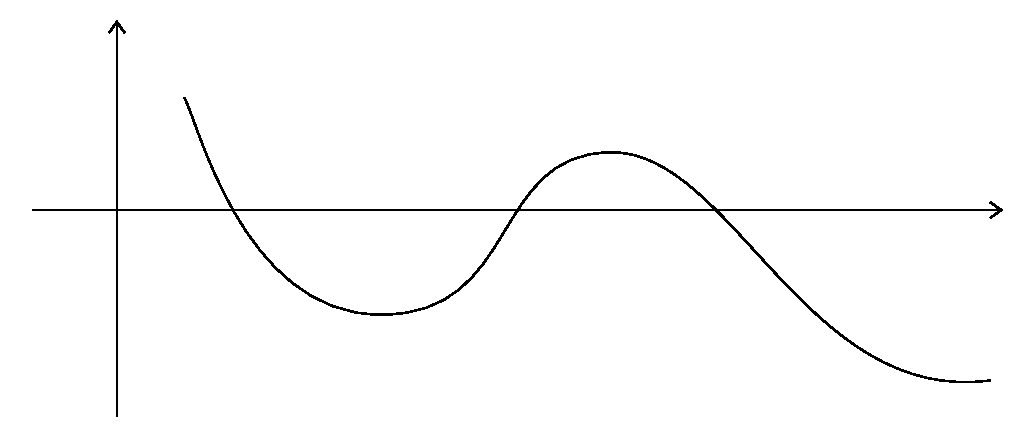
\includegraphics[scale=0.7]{Graph8.pdf}
    \caption{Нежелательное поведение $H(S,T)$}
    \label{nezhelatelnoe_povedenie}
\end{figure}

В таком случае, строгая положительность второй производной $H'_{SS}(S,T)$ позволит избежать возникновения таких случаев. Покажем, что $H'_{SS}(S,T)>0$.

Для простоты, перепишем $H'_S(S,T)$ в более удобном виде: \\ $$H'_S(S,T)=\frac{1}{S^2} \cdot (\ldots)$$. 

В таком случае
\begin{align*}
    & H'_{SS}(S,T) = \left(\frac{1}{S^2} \cdot (\ldots) \right)' = \underbrace{\left(\frac{1}{S^2}\right)'(\ldots)}_{\text{=0}} + \frac{1}{S^2} \cdot \left(\ldots\right)' = \\
    & = \frac{1}{S^2} \left[\frac{2K}{\sigma\sqrt{T}}d_2\varphi(d_2) \frac{1}{S\sigma \sqrt{T}}e^{-rT} +2ae^{-rT}K\frac{1}{S\sigma \sqrt{T}}\varphi(d_2)\right]
\end{align*}

Сравним полученное выражение с нулём. После сокращений получаем, что необходимо, чтобы выполнялось следующее неравенство:
$$ \frac{d_2}{\sigma\sqrt{T}}+a>0$$

Известно, что
$$
\begin{cases}
a = -\frac{\widetilde{\alpha}}{\sigma^2} \\
d_2 = \frac{ln\left(\frac{S}{K}\right)+\widetilde{\alpha}T} {\sigma\sqrt{T}}
\end{cases}
\Rightarrow
\frac{ln\left(\frac{S}{K}\right)+\widetilde{\alpha}T} {(\sigma\sqrt{T})^2} -\frac{\widetilde{\alpha}}{\sigma^2} = \frac{ln\left(\frac{S}{K}\right)}{\sigma^2 T} > 0 
$$

А это верно, поскольку мы считаем, что $S>K$. Следовательно, $H'_S(S,T)=0$,$ H''_{SS}(S,T)>0$, а значит, мы доказали единственность корня. Таким образом, доказаны существование и единственность решения следующего уравнения:
$$ W'_L(S,S) = 0$$

А поскольку корни этого уравнения совпадают с корнями $L(S,0)=S$, то задача построения нижней границы области немедленного исполнения опциона решена.

\newpage
\subsection{Построение графика}

С помощью программы, написанной на языке {\texttt Python} (см. приложение А) удалось построить график, представленный на Рис.~\ref{continuous}, который наглядно отображает вид этой границы. Вдоль оси абсцисс расположено время, а вдоль оси ординат граничное значение для опциона.

\begin{figure}[h]
\centering
\includegraphics[scale=0.6]{Continuous.png}
\caption{Граница области немедленного исполнения в непрерывном случае при \newline $T=2, \sigma=0.3, K=100, S=120, r=0.02, \delta=0.07$}
\label{continuous}
\end{figure} 

\section{Заключение}

В данной работе было рассмотрено построение границы области немедленного исполнения для американского колл-опциона в биномиальной модели рынка. В итоге, были получены результаты для
\begin{enumerate}
    \item Дискретной модели
    \item Непрерывной модели
\end{enumerate}

Дополнительно, был использован метод Ричардсона, который позволил существенно ускорить расчёты в дискретном случае. Был проведён сравнительный анализ классического биномиального метода и метода Ричардсона. Также были построены графики границ в непрерывном и дискретном случаях.

\newpage
\addcontentsline{toc}{section}{Приложение А. Коды программ}
\section*{Приложение А. Коды программ}

\addcontentsline{toc}{subsection}{Построение границы области немедленного исполнения в дискретном случае}
\subsection*{Построение границы области немедленного исполнения в дискретном случае}

\lstset{language=Python}
\begin{lstlisting}
# Libraries
import numpy as np
import matplotlib.pyplot as plt

# Discrete model
T     = 2
si    = 0.3
K     = 100
S     = 120
r     = 0.02
delta = 0.07
n     = 1000

v = np.zeros(2*n+1, dtype=np.float)
s = np.zeros(2*n+1, dtype=np.float)
dt = T / n
r_inv = np.exp(-r*dt)
a  = np.exp((r-delta)*dt)
b2 = a ** 2 * (np.exp(si**2 * dt) - 1)
tmp = a ** 2 + b2 + 1
u = (tmp + np.sqrt(tmp * tmp - 4 * a * a)) / (2*a)
d = 1 / u
p = (a - d)/(u - d)
q = 1 - p
p1 = r_inv * p
q1 = r_inv * q
s[0] = K

for j in range(1,n+1):
    s[j]  = s[j-1] * u
    s[-j] = s[-j+1] * d

for j in range(-n,n+1,2):
    v[j] = max(s[j]-K,0)
    
B_i = []          
for i in range(1, n+1, 1):
    for j in range(-(n-i),(n-i)+1,2):
        v[j] = max(p1 * v[j+1] + q1 * v[j-1], s[j] - K)
    for j in range(-(n-i),(n-i)+1,2):
        if v[j] <= s[j] - K:
            B_i.insert(0,s[j-2])
            break

plt.figure(figsize=(10,5))
plt.plot(B_i)
plt.show()
\end{lstlisting}

\newpage
\addcontentsline{toc}{subsection}{Построение границы области немедленного исполнения в непрерывном случае}
\subsection*{Построение границы области немедленного исполнения в непрерывном случае}

\begin{lstlisting}
# Libraries
import numpy as np
import matplotlib.pyplot as plt
from scipy.optimize import minimize
from scipy.special import erf

# Continuous model
T      = 2
si     = 0.3
K      = 100
S      = 120
r      = 0.02
de     = 0.07
alp    = r-de
alpw   = r-de-si**2/2
bb     = -alpw/si**2
ksi     = np.sqrt(alpw**2+2*r*si**2)
be1    = (-alpw+ksi)/si**2
be2    = (-alpw-ksi)/si**2
Sz     = K*be1/(be1-1)

N = lambda x: (erf(x/np.sqrt(2))+1)/2

b1 = lambda S,L,t: (np.log(S/L)+ksi*t)/(si*np.sqrt(t))
b2 = lambda S,L,t: (np.log(S/L)-ksi*t)/(si*np.sqrt(t))
d1 = lambda S,L,t: (np.log(S/L)+(alpw+si**2)*t)/(si*np.sqrt(t))
d2 = lambda S,L,t: (np.log(S/L)+alpw*t)/(si*np.sqrt(t))

def PW(S,L,t):
    A1 = (1-(L-K)/L*be1)*(S/L)**(be1)*N(b1(S,L,t))
    A2 = (1-(L-K)/L*be2)*(S/L)**(be2)*N(b2(S,L,t))
    A3 = -2*np.exp(-de*t)*(alpw+si**2)/si**2*(S/L)**(2*bb-1)*(N(d1(L**2/S,K,t)) -N(d1(L,S,t)))
    A4 = 2*np.exp(-r*t)*alpw/si**2*K/L*(S/L)**(2*bb)*(N(d2(L**2/S,K,t))-N(d2(L,S,t)))
    return A1+A2+A3+A4

n = 1000
l_nepr = []
for k in range(0, n):
    t = T * (1 - k/n)
    PW_tmp = lambda L1: abs(PW(L1,L1,t))
    res = minimize(PW_tmp, [K], bounds = [(K,Sz)], method='TNC')
    l_nepr.append(res.x[0])
plt.figure(figsize=(10,5))
plt.plot(l_nepr)
plt.xlabel('t')
plt.ylabel('S')
plt.show()
\end{lstlisting}

\newpage
\addcontentsline{toc}{subsection}{Классический биномиальный метод}
\subsection*{Классический биномиальный метод}

\begin{lstlisting}
# Libraries
import numpy as np
import time

def classic_bin(S, K, T, sigma, r, delta, n, res):
    
    start_time = time.time()
    
    # Initialize parameters
    v = np.zeros(2*n+1, dtype=np.float)
    s = np.zeros(2*n+1, dtype=np.float)
    dt = T / n
    r_inv = np.exp(-r*dt)
    a  = np.exp((r-delta)*dt)
    b2 = a ** 2 * (np.exp(sigma * sigma * dt) - 1)
    tmp = a ** 2 + b2 + 1
    u = (tmp + np.sqrt(tmp * tmp - 4 * a * a)) / (2*a)
    d = 1 / u
    p = (a - d)/(u - d)
    q = 1 - p
    p1 = r_inv * p
    q1 = r_inv * q
    s[0] = S

    # The level to calculate the bound for
    level = 2*n//3 
    
    for j in range(1,n+1):
        s[j]  = s[j-1] * u
        s[-j] = s[-j+1] * d

    # Store option values at time index i = n
    for j in range(-n,n+1,2):
        v[j] = max(s[j]-K,0)

    # Work backwards in time
    for i in range(n-1, -1, -1):
        for j in range(-i,i+1,2):
            v[j] = max(p1 * v[j+1] + q1 * v[j-1], s[j] - K)
            
    # Getting the bound
    for j in range(level+1,-level,-1):
        if (v[j] > s[j] - K):
            bound = s[j]
            break

    # Return binomial option value
    C = v[0]
    finish_time = time.time()
    print("%.3f" % C, "  ", "%.3f" % res, ' --- ', bound, ', ===', finish_time-start_time)
\end{lstlisting}

\newpage
\addcontentsline{toc}{subsection}{Метод Ричардсона}
\subsection*{Метод Ричардсона}

\begin{lstlisting}
# Libraries
import numpy as np
import time

def P1(S, K, T, sigma, r, delta, n):
    # Initialize parameters
    v = np.zeros(2*n+1, dtype=np.float)
    s = np.zeros(2*n+1, dtype=np.float)
    b = np.zeros(2*n+1, dtype=np.float)
    vtmp = np.zeros(2*n+1, dtype=np.float)
    dt = T / n
    r_inv = np.exp(-r*T) # (!) changed here
    a  = np.exp((r-delta)*dt)
    b2 = a ** 2 * (np.exp(sigma * sigma * dt) - 1)
    tmp = a ** 2 + b2 + 1
    u = (tmp + np.sqrt(tmp * tmp - 4 * a * a)) / (2*a)
    d = 1 / u
    p = (a - d)/(u - d)
    q = 1 - p
    s[0] = S


    for j in range(2,n+1,2):
        s[j]  = s[j-2] * u*u
        s[-j] = s[-j+2] * d*d

    # Store option values at time index i = n
    for j in range(-n,n+1,2):
        v[j] = max(s[j]-K,0)

    # Store binomial terms
    m = n # (!) changed here 
    b[m] = p**m
    for j in range(1,m+1):
        k = m - 2*j
        b[k] = b[k+2] * ((m-j+1)/j)*(q/p)

    # Evaluate at time i=0
    sumproduct = 0
    for k in range(-m,m+1,2):
        sumproduct += b[k]*v[k]
    vtmp[0] = r_inv * sumproduct

    # Return P(1) value
    P_1 = vtmp[0]
    return P_1
    
def P2(S, K, T, sigma, r, delta, n):
    # Initialize parameters
    v = np.zeros(2*n+1, dtype=np.float)
    s = np.zeros(2*n+1, dtype=np.float)
    b = np.zeros(2*n+1, dtype=np.float)
    vtmp = np.zeros(2*n+1, dtype=np.float)
    dt = T / n
    r_inv = np.exp(-r*T/2) # (!) changed here
    a  = np.exp((r-delta)*dt)
    b2 = a ** 2 * (np.exp(sigma * sigma * dt) - 1)
    tmp = a ** 2 + b2 + 1
    u = (tmp + np.sqrt(tmp * tmp - 4 * a * a)) / (2*a)
    d = 1 / u
    p = (a - d)/(u - d)
    q = 1 - p
    s[0] = S


    for j in range(2,n+1,2):
        s[j]  = s[j-2] * u*u
        s[-j] = s[-j+2] * d*d

    # Store option values at time index i = n
    for j in range(-n,n+1,2):
        v[j] = max(s[j]-K,0)

    # Store binomial terms
    m = n // 2 # (!) changed here 
    b[m] = p**m
    for j in range(1,m+1):
        k = m - 2*j
        b[k] = b[k+2] * ((m-j+1)/j)*(q/p)

    # Evaluate at time index i=n/2=m
    for j in range(-m, m+1, 2):
        # sumproduct(b[2k-m],v[2k-m+j], k=0 to m by 1)
        sumproduct = 0
        for k in range(0,m+1):
            sumproduct += b[2*k-m] * v[2*k-m+j]
        vtmp[j] = sumproduct    
        vtmp[j] = max(r_inv*vtmp[j], s[j]-K)

    for j in range(-m,m+1,2):
        v[j] = vtmp[j]

    # Evaluate at time i=0
    sumproduct = 0
    for k in range(-m,m+1,2):
        sumproduct += b[k]*v[k]
    vtmp[0] = r_inv * sumproduct

    # Return P(2) value
    P_2 = vtmp[0]
    return P_2
    
def P3(S, K, T, sigma, r, delta, n):
    # Initialize parameters
    v = np.zeros(2*n+1, dtype=np.float)
    s = np.zeros(2*n+1, dtype=np.float)
    b = np.zeros(2*n+1, dtype=np.float)
    vtmp = np.zeros(2*n+1, dtype=np.float)
    dt = T / n
    r_inv = np.exp(-r*T/3)
    a  = np.exp((r-delta)*dt)
    b2 = a ** 2 * (np.exp(sigma * sigma * dt) - 1)
    tmp = a ** 2 + b2 + 1
    u = (tmp + np.sqrt(tmp * tmp - 4 * a * a)) / (2*a)
    d = 1 / u
    p = (a - d)/(u - d)
    q = 1 - p
    s[0] = S


    for j in range(2,n+1,2):
        s[j]  = s[j-2] * u*u
        s[-j] = s[-j+2] * d*d

    # Store option values at time index i = n
    for j in range(-n,n+1,2):
        v[j] = max(s[j]-K,0)

    # Store binomial terms
    m = n // 3 
    b[m] = p**m
    for j in range(1,m+1):
        k = m - 2*j
        b[k] = b[k+2] * ((m-j+1)/j)*(q/p)

    # Evaluate at time index i=2n/3=2m
    for j in range(-2*m, 2*m+1, 2):
        # sumproduct(b[2k-m],v[2k-m+j], k=0 to m by 1)
        sumproduct = 0
        for k in range(0,m+1):
            sumproduct += b[2*k-m] * v[2*k-m+j]
        vtmp[j] = sumproduct    
        vtmp[j] = max(r_inv*vtmp[j], s[j]-K)

    for j in range(-m,m+1,2):
        v[j] = vtmp[j]

    # Evaluate at time index i=n/3=m
    for j in range(-m, m+1, 2):
        # sumproduct(b[2k-m],v[2k-m+j], k=0 to m by 1)
        sumproduct = 0
        for k in range(0,m+1):
            sumproduct += b[2*k-m] * v[2*k-m+j]
        vtmp[j] = sumproduct    
        vtmp[j] = max(r_inv*vtmp[j], s[j]-K)

    for j in range(-m,m+1,2):
        v[j] = vtmp[j]

    # Evaluate at time i=0
    sumproduct = 0
    for k in range(-m,m+1,2):
        sumproduct += b[k]*v[k]
    vtmp[0] = r_inv * sumproduct

    # Return P(3) value
    P_3 = vtmp[0]
    return vtmp[0]
    
def richardson_bin(S, K, T, sigma, r, delta, n, res):
    start_time = time.time()
    P_1 = P1(S, K, T, sigma, r, delta, n)
    P_2 = P2(S, K, T, sigma, r, delta, n)
    P_3 = P3(S, K, T, sigma, r, delta, n)
    finish_time = time.time()
    t = finish_time - start_time

    val = P_3 + 3.5*(P_3 - P_2) - 0.5*(P_2 - P_1)
    print("%.3f" % val, "  ", "%.3f" % res, '===', "%.3f" % t)
    return
\end{lstlisting}

% Список литературы
\newpage
\addcontentsline{toc}{section}{Список литературы}
\begin{thebibliography}{}
	\bibitem{cox} 	Cox J., Ross S.A., Rubinstein M. Option Pricing: A Simplified Approach // Journal of Financial Economics. 1979. V. 7, № 3. P. 229-263.
	\bibitem{broadie} Broadie M., Detemple J. American Option Valuation: New Bounds, Approximations, and a Comparison of Existing Methods // The Review of Financial Studies. 1996. V. 9, № 4. P. 1211-1250.
    \bibitem{geske} Geske R., Johnson H. E. The American Put Option Valued Analytically // The Journal of Finance. 1984. V. 39, № 5. P. 1511-1524.
    \bibitem{hull} Hull J., White A. The Use of the Control Variate Technique in Option Pricing // The Journal of Financial and Quantitative Analysis. 1988. V. 23, № 3. P. 237-251.
\end{thebibliography}


\end{document}


